\documentclass[10pt, aspectratio=169]{beamer}

% ═══════════════════════════════════════════════════════════════════════════
%  Professional Academic Theme — IIT Delhi branding
% ═══════════════════════════════════════════════════════════════════════════

% ── Theme ───────────────────────────────────────────────────────────────────
\usetheme{Madrid}
\useinnertheme{rectangles}
\beamertemplatenavigationsymbolsempty

% ── Colour Palette ─────────────────────────────────────────────────────────
\definecolor{iitdNavy}{HTML}{003B5C}
\definecolor{iitdDark}{HTML}{002642}
\definecolor{iitdAccent}{HTML}{0077B6}
\definecolor{iitdGray}{HTML}{4A5568}
\definecolor{iitdLightGray}{HTML}{E2E8F0}
\definecolor{alertRed}{HTML}{B91C1C}
\definecolor{successGreen}{HTML}{047857}

% ── Apply colours ──────────────────────────────────────────────────────────
\setbeamercolor{palette primary}{bg=iitdNavy, fg=white}
\setbeamercolor{palette secondary}{bg=iitdDark, fg=white}
\setbeamercolor{palette tertiary}{bg=iitdDark, fg=white}
\setbeamercolor{palette quaternary}{bg=iitdNavy, fg=white}
\setbeamercolor{structure}{fg=iitdNavy}
\setbeamercolor{frametitle}{bg=iitdNavy, fg=white}
\setbeamercolor{title}{fg=white, bg=iitdNavy}
\setbeamercolor{subtitle}{fg=iitdLightGray}
\setbeamercolor{author}{fg=white}
\setbeamercolor{institute}{fg=iitdLightGray}
\setbeamercolor{date}{fg=iitdLightGray}
\setbeamercolor{normal text}{fg=iitdGray}
\setbeamercolor{alerted text}{fg=alertRed}
\setbeamercolor{example text}{fg=successGreen}
\setbeamercolor{block title}{bg=iitdNavy, fg=white}
\setbeamercolor{block body}{bg=iitdLightGray!40, fg=iitdGray}
\setbeamercolor{block title alerted}{bg=alertRed!85!black, fg=white}
\setbeamercolor{block body alerted}{bg=alertRed!8, fg=iitdGray}
\setbeamercolor{block title example}{bg=successGreen!85!black, fg=white}
\setbeamercolor{block body example}{bg=successGreen!8, fg=iitdGray}
\setbeamercolor{itemize item}{fg=iitdNavy}
\setbeamercolor{itemize subitem}{fg=iitdAccent}
\setbeamercolor{enumerate item}{fg=iitdNavy}

% ── Fonts ──────────────────────────────────────────────────────────────────
\setbeamerfont{title}{size=\Large, series=\bfseries}
\setbeamerfont{frametitle}{size=\large, series=\bfseries}
\setbeamerfont{block title}{size=\normalsize, series=\bfseries}

% ── Bullets ────────────────────────────────────────────────────────────────
\setbeamertemplate{itemize item}{\small$\bullet$}
\setbeamertemplate{itemize subitem}{\scriptsize$\circ$}

% ── Footer ─────────────────────────────────────────────────────────────────
\setbeamertemplate{footline}{%
  \hfill%
  \usebeamercolor[fg]{normal text}%
  \usebeamerfont{footline}%
  \footnotesize\insertframenumber\,/\,\inserttotalframenumber%
  \hspace{8pt}\vspace{4pt}%
}

% ── Packages ───────────────────────────────────────────────────────────────
\usepackage{graphicx}
\usepackage{booktabs}
\usepackage[table]{xcolor}
\usepackage{amsmath,amssymb}
\usepackage{siunitx}
\usepackage{tikz}
\usetikzlibrary{positioning}
\usepackage{hyperref}
\usepackage{multicol}
\usepackage{caption}
\captionsetup{font=small, labelformat=empty}

\graphicspath{{assets/}{logos/}}

% ── Key Insight box ────────────────────────────────────────────────────────
\newcommand{\keyinsight}[1]{%
  \begin{beamercolorbox}[wd=\textwidth, sep=6pt, rounded=true]{block body}
    \textcolor{iitdNavy}{\textbf{\small$\star$\;Key Insight:}}\;
    {\small #1}
  \end{beamercolorbox}%
}

% ═══════════════════════════════════════════════════════════════════════════
\begin{document}

% ─── SLIDE 1: TITLE ──────────────────────────────────────────────────────────
\begin{frame}[plain]
    \begin{tikzpicture}[remember picture, overlay]
        \shade[left color=iitdDark, right color=iitdAccent!80!iitdNavy,
               shading angle=15]
            (current page.south west) rectangle (current page.north east);
        \fill[white, opacity=0.06]
            ([xshift=-2cm, yshift=-2.5cm]current page.north east) circle (6cm);
        \fill[white, opacity=0.04]
            ([xshift=2.5cm, yshift=2cm]current page.south west) circle (4.5cm);
        \draw[iitdAccent!60!white, line width=0.8pt]
            ([xshift=2cm, yshift=-0.5cm]current page.west)
            -- ([xshift=-2cm, yshift=-0.5cm]current page.east);

        \node[anchor=south, text width=0.85\paperwidth, align=center]
            at ([yshift=1.0cm]current page.center) {
                {\LARGE\bfseries\color{white}%
                 Multiobjective Optimization of Hydrogen\\[6pt]
                 Injection into Natural Gas Pipelines}\\[14pt]
                {\large\color{iitdLightGray}A Surrogate-Assisted Approach }\\[14pt]
                {\large\color{iitdAccent!80!white}\textbf{CLD880 -- Minor Project Presentation}}
            };

        \node[anchor=north, text width=0.75\paperwidth, align=center]
            at ([yshift=-1.2cm]current page.center) {
                {\large\color{white}\textbf{Sakhare Yash Balram}\;\;{\normalsize (2022CH71496)}}\\[8pt]
                {\large\color{iitdLightGray}%
                 Supervisor: \textbf{Prof.\ Abhijeet Raj}}\\[6pt]
                {\normalsize\color{iitdLightGray}%
                 Department of Chemical Engineering\\
                 Indian Institute of Technology Delhi}\\[10pt]
                {\small\color{iitdLightGray!80}February 2026}
            };
    \end{tikzpicture}
\end{frame}

% ═══════════════════════════════════════════════════════════════════════════
\section{Introduction}
% ═══════════════════════════════════════════════════════════════════════════

% ─── SLIDE 2: INTRODUCTION ─────────────────────────────────────
\begin{frame}{Introduction}
    \begin{columns}[T]
        \begin{column}{0.55\textwidth}
            \textbf{Power-to-Gas (P2G) Transition:}
            \begin{itemize}
                \item \textbf{Fuel Replacement:} Blending Green H$_2$ into Natural Gas decarbonizes the energy mix, acting as a vital clean transition fuel.
                \item \textbf{Infrastructure Synergy:} Escapes the high CAPEX of new pipelines by re-using existing gas infrastructure.
                \item Crucial for early-stage hydrogen economy adoption.
            \end{itemize}

            \vspace{0.4em}
            \textbf{The Physical Challenge:}
            \begin{itemize}
                \item H$_2$ is \textbf{$\sim$1/8th} the density of CH$_4$ ($0.082$ vs $0.668$ kg/m$^3$).
                \item High density deficit causes buoyancy-driven \alert{stratification} (H$_2$ flows at the pipe crown).
            \end{itemize}
        \end{column}
        \begin{column}{0.42\textwidth}
            \begin{alertblock}{Risks of Poor Mixing}
                \small
                \begin{itemize}
                    \item \textbf{Hydrogen Embrittlement} at the pipe crown due to localized high partial pressures.
                    \item \textbf{Wobbe Index drift} causing combustion instability in end-user turbines.
                    \item \textbf{Metering errors} due to variation in the speed of sound.
                \end{itemize}
            \end{alertblock}
            
            \vspace{0.2em}
            \keyinsight{Achieving a uniform mixture safely and economically is the primary operational hurdle in H$_2$ blending.}
        \end{column}
    \end{columns}
\end{frame}

% ─── SLIDE 3: THE FUNDAMENTAL ENGINEERING CHALLENGE ──────────────────────────
\begin{frame}{The Fundamental Engineering Challenge}
    \begin{columns}[T]
        \begin{column}{0.52\textwidth}
            Designing a T-junction injector requires balancing two \textbf{conflicting objectives}:
            
            \vspace{0.4em}
            \begin{table}
                \centering
                \scriptsize
                \begin{tabular}{@{}p{0.46\textwidth}p{0.46\textwidth}@{}}
                    \toprule
                    \cellcolor{green!15}\textbf{$\uparrow$ Maximize Safety} &
                    \cellcolor{red!15}\textbf{$\downarrow$ Minimize Cost} \\
                    \midrule
                    Metric: \textbf{CoV} (Mixing Quality) & Metric: \textbf{$\Delta P$} (Energy Loss) \\[4pt]
                    Requires high turbulence, counter-flow arrays (\alert{increases pressure loss}) & Requires smooth co-flow injection (\alert{reduces mixing efficiency}) \\
                    \bottomrule
                \end{tabular}
            \end{table}

            \vspace{0.2em}
            \begin{block}{}
                \centering
                \small
                \alert{Improving mixing inherently degrades operational cost.}
            \end{block}
        \end{column}
        \begin{column}{0.45\textwidth}
            \vspace{1.5em}
            \begin{center}
                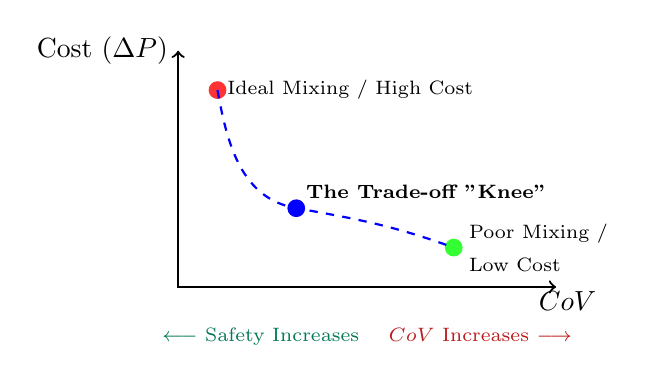
\begin{tikzpicture}
                    % Axes
                    \draw[<->, thick] (0,3) node[left] {Cost ($\Delta P$)} -- (0,0) -- (4.8,0) node[below right, xshift=-10pt, yshift=2pt] {$CoV$};
                    \node[below, align=center] at (2.4, -0.4) {\scriptsize \textcolor{successGreen}{$\longleftarrow$ Safety Increases} \quad \textcolor{alertRed}{$CoV$ Increases $\longrightarrow$}};
                    
                    % Points
                    \filldraw[red!80] (0.5,2.5) circle (3pt) node[right, black] {\scriptsize Ideal Mixing / High Cost};
                    \filldraw[green!80] (3.5,0.5) circle (3pt) node[right, black, align=left, xshift=2pt] {\scriptsize Poor Mixing /\\ \scriptsize Low Cost};
                    
                    % Curve
                    \draw[thick, dashed, blue] (0.5,2.5) to[out=280,in=170] (1.5,1.0) to[out=350,in=160] (3.5,0.5);
                    
                    % Knee Point
                    \filldraw[blue] (1.5,1.0) circle (3pt) node[above right, black] {\scriptsize \textbf{The Trade-off "Knee"}};
                \end{tikzpicture}
            \end{center}
        \end{column}
    \end{columns}
\end{frame}

% ═══════════════════════════════════════════════════════════════════════════
\section{Literature Review \& The Gap}
% ═══════════════════════════════════════════════════════════════════════════

% ─── SLIDE 4: LITERATURE REVIEW (WHAT HAS BEEN DONE) ─────────────────────────
\begin{frame}{Literature Review: What has been done?}
    \begin{columns}[T]
        \begin{column}{0.5\textwidth}
            \textbf{1. Mixing Quality ($CoV$) Studies (Su, Azman):}
            \begin{itemize}
                \small
                \item Focused purely on minimizing CoV.
                \item Finding: Counter-flow ($\theta > 90^\circ$) and high velocity ratios ($R_v$) yield the best homogeneity.
                \item \alert{Issue:} Complete disregard for the energy expenditure ($\Delta P$) required.
            \end{itemize}

            \vspace{0.4em}
            \textbf{2. Cost ($\Delta P$) Studies (He, Zhang):}
            \begin{itemize}
                \small
                \item Focused on pipeline network pumping costs.
                \item Finding: Co-flow injection minimizes pressure drops.
                \item \alert{Issue:} Assumes perfect mixing occurs instantaneously, ignoring safety risks.
            \end{itemize}
        \end{column}
        \begin{column}{0.48\textwidth}
            \textbf{3. Machine Learning Applications:}
            \begin{itemize}
                \small
                \item Recent adoptions of ML (e.g., Su et al., 2022).
                \item \alert{Issue:} ML models treat mixing exclusively as a single-output prediction task ($\widehat{CoV}$).
            \end{itemize}

            \vspace{0.8em}
            \textbf{4. Network-Level MOO (Arya et al., 2023):}
            \begin{itemize}
                \small
                \item Successfully applied multi-objective optimization to macroscopic hydrogen-natural gas network routing.
                \item \alert{Issue:} Assumes perfect mixing at injection sites; ignores the complex microscopic fluid dynamics and local pressure penalties at the T-junction itself.
            \end{itemize}
        \end{column}
    \end{columns}
\end{frame}

% ─── SLIDE 5: THE EXPLICIT RESEARCH GAP ──────────────────────────────────────
\begin{frame}{The Explicit Research Gap}
    \begin{center}
        \Large \alert{\textbf{"No study to date has performed a simultaneous Multi-Objective Optimization on the injection geometry"}}
    \end{center}
    
    \vspace{0.8em}
    \begin{columns}[T]
        \begin{column}{0.5\textwidth}
            \textbf{Why does this gap exist?}
            \begin{enumerate}
                \small
                \item \textbf{Data Fragmentation:} $CoV$ and $\Delta P$ are rarely extracted simultaneously in literature.
                \item \textbf{Computational Setup:} Real-world MOO requires tens of thousands of function evaluations.
                \begin{itemize}
                    \scriptsize
                    \item 1 CFD run $\approx$ 3-4 hours.
                    \item $30,000$ runs $\approx$ \textbf{10 years} of compute.
                \end{itemize}
            \end{enumerate}
        \end{column}
        \begin{column}{0.5\textwidth}
            \textbf{Why is filling this gap critical?}
            \begin{itemize}
                \small
                \item Without a \textbf{Pareto Frontier}, pipeline operators cannot make informed, quantitative decisions on the safety vs. cost trade-off.
                \item T-junctions are the most common, cheapest injection method - optimizing them passively saves extensive CAPEX.
            \end{itemize}
        \end{column}
    \end{columns}
\end{frame}

% ═══════════════════════════════════════════════════════════════════════════
\section{Proposed Solution}
% ═══════════════════════════════════════════════════════════════════════════

% ─── SLIDE 6: PROPOSED SOLUTION ─────────────────────────
\begin{frame}{Proposed Solution}
    \begin{columns}[T]
        \begin{column}{0.45\textwidth}
            \vspace{0.5em}
            \textbf{AI-Assisted Framework:} \\
            Developing the \textbf{first surrogate-assisted optimization framework} capable of mapping the full Pareto front for hydrogen blending geometries.
            
            \vspace{0.8em}
            \textbf{How it differs:}
            \begin{itemize}
                \small
                \item \textbf{Multi-Output:} Predicting both $CoV$ and $\Delta P$ simultaneously.
                \item \textbf{Buoyancy Focus:} Explicitly comparing "Top" vs "Bottom" injection.
            \end{itemize}
        \end{column}
        \begin{column}{0.52\textwidth}
            \textbf{The 4-Step Technical Approach:}
            \begin{center}
                \vspace{0.2em}
                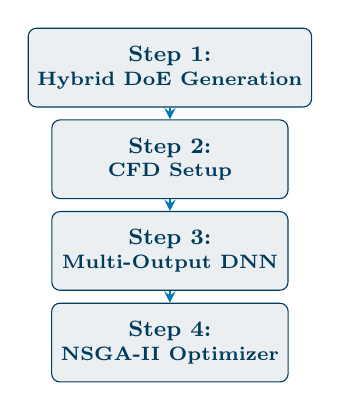
\begin{tikzpicture}[
                    wfbox/.style={draw=iitdNavy, fill=iitdNavy!8, rounded corners=3pt,
                                  minimum height=1.0cm, minimum width=3.0cm, align=center,
                                  font=\footnotesize\bfseries, text=iitdNavy},
                    arr/.style={->, >=stealth, thick, color=iitdAccent},
                    node distance=0.15cm
                ]
                    \node[wfbox] (s1) {Step 1:\\[-1pt]{\scriptsize Hybrid DoE Generation}};
                    \node[wfbox, below=of s1] (s2) {Step 2:\\[-1pt]{\scriptsize CFD Setup}};
                    \node[wfbox, below=of s2] (s3) {Step 3:\\[-1pt]{\scriptsize Multi-Output DNN}};
                    \node[wfbox, below=of s3] (s4) {Step 4:\\[-1pt]{\scriptsize NSGA-II Optimizer}};
                    \draw[arr] (s1) -- (s2);
                    \draw[arr] (s2) -- (s3);
                    \draw[arr] (s3) -- (s4);
                \end{tikzpicture}
            \end{center}
        \end{column}
    \end{columns}
\end{frame}

% ─── SLIDE 7: PROBLEM FORMULATION ────────────────────────────────────────────
\begin{frame}{Problem Formulation}
    \begin{columns}[T]
        \begin{column}{0.48\textwidth}
            \textbf{Design Variables ($\mathbf{x}$):}
            \begin{table}
                \centering
                \scriptsize
                \begin{tabular}{@{}ll@{}}
                    \toprule
                    \textbf{Variable} & \textbf{Range} \\
                    \midrule
                    Position ($P_{\text{inj}}$) & \textbf{Top} vs. \textbf{Bottom} \\
                    Angle ($\theta$) & 30\textdegree-150\textdegree \\
                    Diam.\ ratio ($\beta$) & 0.1-0.5 \\
                    Vel.\ ratio ($R_v$) & 0.5-4.0 \\
                    Blend ratio ($HBR$) & 5\%-30\% \\
                    \bottomrule
                \end{tabular}
            \end{table}
            
            \textbf{Constraints:}
            \begin{itemize}
                \scriptsize
                \item $5\% \leq HBR \leq 30\%$ (Safe operational limit)
                \item Target: $CoV_{50D} < 0.05$ (Engineering standard for "mixed")
            \end{itemize}
        \end{column}
        \begin{column}{0.48\textwidth}
            \textbf{Formal MOO Statement:}
            \[
                \min_{\mathbf{x}} \;
                \mathbf{F}(\mathbf{x}) = \begin{bmatrix}
                    CoV_{50D}(\mathbf{x}) \\[4pt]
                    \Delta P(\mathbf{x})
                \end{bmatrix}
            \]
            
            \vspace{0.6em}
            \begin{block}{The Objective}
                Determine the specific combinations of $[\theta, \beta, R_v]$ for both Top and Bottom injections that yield points on the \textbf{Pareto Boundary}.
            \end{block}
        \end{column}
    \end{columns}
\end{frame}

% ═══════════════════════════════════════════════════════════════════════════
% ═══════════════════════════════════════════════════════════════════════════
\section{Solution Framework}
% ═══════════════════════════════════════════════════════════════════════════

% ─── SLIDE 8: FRAMEWORK STEP 1 (Hybrid DoE) ──────────────────────────────────
\begin{frame}{Framework Step 1: Hybrid DoE Generation}
    \begin{columns}[T]
        \begin{column}{0.48\textwidth}
            \textbf{Constructing the Experimental Dataset}
            \begin{itemize}
                \item \textbf{Goal:} Create a space-filling, representative dataset to train the multi-output surrogate.
                \item \textbf{Hybrid Sampling Strategy:} 
                  \begin{itemize}
                      \small
                      \item \textbf{15} distinct geometric meshes (varying $\theta, \beta$).
                      \item \textbf{14} Latin Hypercube Samples (LHS) per mesh for flow boundary conditions ($R_v, HBR$).
                      \item Evaluated for \textbf{2} Injection Positions (Top, Bottom).
                  \end{itemize}
                \item \textbf{Total Yield:} \textbf{420 distinct structural cases}.
            \end{itemize}
        \end{column}
        \begin{column}{0.50\textwidth}
            \begin{figure}
                \centering
                \includegraphics[width=0.85\linewidth]{doe_diagnostics_discrete.png}
                \caption{LHS continuous sampling distribution ensuring no clustering in the operational parameter space.}
            \end{figure}
        \end{column}
    \end{columns}
\end{frame}

% ─── SLIDE 9: FRAMEWORK STEP 2 (CFD Setup) ───────────────────────────────────
\begin{frame}{Framework Step 2: CFD Setup (Basis)}
    \begin{columns}[T]
        \begin{column}{0.55\textwidth}
            \textbf{1. Physics \& Operating Conditions}
            \begin{itemize}
                \scriptsize
                \item\textbf{Pressure:} \textbf{3.5 MPa} (Pipeline operating condition)
                \item\textbf{Temperature:} \textbf{288 K} (Ambient)
                \item\textbf{Species transport:} Enabled to track $\text{H}_2$ \& $\text{CH}_4$ mixing
                \item\textbf{Turbulence model:} Realizable $k$--$\varepsilon$ (Validated against LES and $k$--$\omega$ SST)
                \item\textbf{Equation of State:} Peng-Robinson (vital to accurately capture density difference and compressibility)
            \end{itemize}
            
            \vspace{0.4em}
            \textbf{2. Mixing Uniformity Metric}
            \begin{itemize}
                \scriptsize
                \item \textbf{Coefficient of Variation ($CoV$)} of $\text{H}_2$ concentration across cross-sections:
                \[ CoV = \frac{\sigma}{\bar{c}} = \frac{\sqrt{\frac{1}{A} \int_A (c_i - \bar{c})^2 dA}}{\bar{c}} \]
                \item Evaluated up to $L = 50D$ downstream.
            \end{itemize}
        \end{column}
        \begin{column}{0.40\textwidth}
            \begin{figure}
                \centering
                \includegraphics[width=0.9\linewidth]{mesh.png}
                \vspace{-0.2em}
                \caption{Hexahedral mesh near the T-junction\\(Adapted from Su et al.)}
            \end{figure}
        \end{column}
    \end{columns}
\end{frame}

% ─── SLIDE 10: FRAMEWORK STEP 3 (SYNTHETIC OUTPUT DATA & DNN) ───────────────────────
\begin{frame}{Framework Step 3: Synthetic Output Data \& Surrogate Modeling}
    \begin{columns}[T]
        \begin{column}{0.50\textwidth}
            \textbf{3. Pipeline Validation (Synthetic Output Data)}
            
            \vspace{0.8em}
            \textbf{Synthetic Models Used:}
            {\scriptsize
            \begin{align*}
                CoV_{\text{syn}} &\propto (0.05 + 0.15\,R_v^{0.8})(1 - 0.35\sin\theta)\cdots \\
                \Delta P_{\text{syn}} &= K(\theta, \beta) \cdot \tfrac{1}{2}\rho_{NG} v_{\text{jet}}^2
            \end{align*}}

            \vspace{0.4em}
            \keyinsight{All results that follow use this synthetic data. The modular pipeline requires \textbf{zero code changes} when the real CFD data arrives.}
            
            \vfill
            {\tiny \textcolor{gray}{\textit{*Note: CFD simulations take time to generate actual outputs; to test the pipeline in the interim, this synthetic data was generated.}}}
        \end{column}
        \begin{column}{0.48\textwidth}
            \textbf{4. Deep Neural Network (DNN)}
            \begin{center}
                \includegraphics[width=0.95\linewidth]{dnn_architecture.png}
            \end{center}

            \vspace{-0.4em}
            \begin{table}
                \centering
                \scriptsize
                \begin{tabular}{@{}ll@{}}
                    \toprule
                    \textbf{Config} & \textbf{Value} \\
                    \midrule
                    Loss & MSE + $L_2$ ($\alpha\!=\!10^{-4}$) \\
                    Optimizer & Adam ($\eta\!=\!0.001$) \\
                    Params & $\sim$17,410 (4 Hidden Layers) \\
                    Train/Val/Test & 68\% / 12\% / 20\% \\
                    \bottomrule
                \end{tabular}
            \end{table}
        \end{column}
    \end{columns}
\end{frame}

% ─── SLIDE 11: FRAMEWORK STEP 4 (NSGA-II) ────────────────────────────────────
\begin{frame}{Framework Step 4: NSGA-II Optimization}
    \begin{columns}[T]
        \begin{column}{0.55\textwidth}
            \textbf{5. Evolutionary Optimization}
            \begin{itemize}
                \item Algorithm: \textbf{NSGA-II} (Non-dominated Sorting Genetic Algorithm II)
                \item Widely used for highly non-linear, multi-modal problems.
            \end{itemize}

            \vspace{0.3em}
            \textbf{Algorithm Configuration:}
            \begin{table}
                \centering
                \small
                \begin{tabular}{@{}lc@{}}
                    \toprule
                    \textbf{Parameter} & \textbf{Value} \\
                    \midrule
                    Population size ($N$)  & 200 \\
                    Generations ($G$)      & 150 \\
                    Crossover & SBX ($\eta_c = 15$, $p_c = 0.9$) \\
                    Mutation  & Polynomial ($\eta_m = 20$) \\
                    \bottomrule
                \end{tabular}
            \end{table}
        \end{column}
        \begin{column}{0.42\textwidth}
            \vspace{1.5em}
            \begin{alertblock}{The Surrogate Advantage}
                \centering
                200 pop $\times$ 150 gens = \textbf{30,000 evaluations}.\\
                \vspace{0.5em}
                Takes \textbf{$<$30 seconds} with the DNN. \\
                \vspace{0.5em}
                Direct CFD-in-the-loop would take \textbf{$\sim$10 years}.
            \end{alertblock}
            
            \vspace{0.5em}
            \keyinsight{This computational speedup is what makes identifying the Pareto Frontier possible.}
        \end{column}
    \end{columns}
\end{frame}

% ═══════════════════════════════════════════════════════════════════════════
\section{Preliminary Results}
% ═══════════════════════════════════════════════════════════════════════════

% ─── SLIDE 12: SURROGATE ACCURACY ────────────────────────────────────────────
\begin{frame}{Preliminary Results: Surrogate Accuracy}
    \begin{alertblock}{}
        \centering
        \small
        \textbf{Note:} Results generated via end-to-end pipeline validation using \textit{literature-calibrated synthetic data}.
    \end{alertblock}

    \vspace{1.5em}
    \begin{figure}
        \centering
        \includegraphics[width=0.85\linewidth]{dnn_parity.png}
        \caption{Parity plots: predicted vs.\ actual for CoV and $\Delta P$}
    \end{figure}
\end{frame}

% ─── SLIDE 13: PARETO FRONTIER ───────────────────────────────────────────────
\begin{frame}{Preliminary Results: The Pareto Frontier}
    \begin{columns}[T]
        \begin{column}{0.52\textwidth}
            \begin{figure}
                \centering
                \includegraphics[width=\linewidth]{pareto_front.png}
                \caption{Pareto fronts for Top \& Bottom injection (synthetic data)}
            \end{figure}
        \end{column}
        \begin{column}{0.44\textwidth}
            \textbf{Mapping the Trade-off}
            \begin{enumerate}
                \item \textbf{Clear Conflicting Behavior:} Lowering CoV undeniably increases $\Delta P$.
                \item \textbf{Bottom Dominates Top:} The Bottom injection front lies to the "bottom-left" (better) of Top injection. Buoyancy naturally assists mixing.
                \item \textbf{Three Regions:}
                    \begin{itemize}
                        \item \textbf{A:} Poor mixing, cheap to operate.
                        \item \textbf{B:} Excellent mixing, exorbitant OPEX.
                        \item \textbf{Knee:} The optimal engineering compromise.
                    \end{itemize}
            \end{enumerate}
        \end{column}
    \end{columns}
\end{frame}

% ═══════════════════════════════════════════════════════════════════════════
\section{Impact \& Future Work}
% ═══════════════════════════════════════════════════════════════════════════



% ─── SLIDE 14: PROGRESS & FUTURE WORK ────────────────────────────────────────
\begin{frame}{Current Progress \& Future Work}
    \begin{columns}[T]
        \begin{column}{0.45\textwidth}
            \textbf{\textcolor{successGreen}{$\checkmark$}\; Current Progress}
            \vspace{2.2em}
            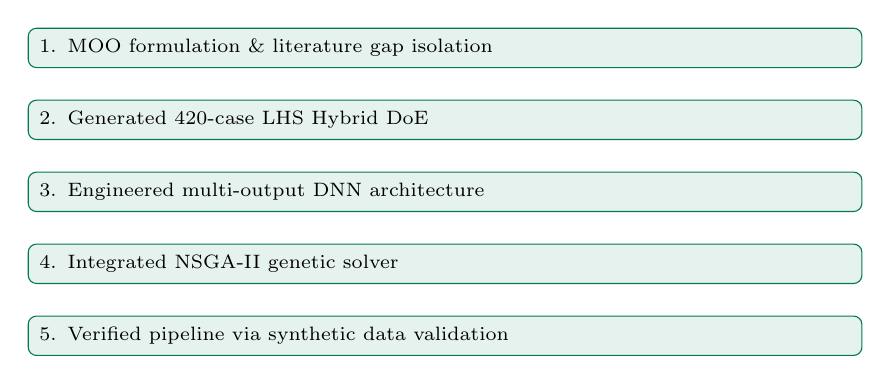
\begin{tikzpicture}[
                node distance=0.4cm,
                chkbox/.style={fill=successGreen!10, draw=successGreen, rounded corners=3pt,
                               text width=0.85\linewidth, align=left, font=\scriptsize,
                               inner sep=4pt}
            ]
                \node[chkbox] (c1) {1. MOO formulation \& literature gap isolation};
                \node[chkbox, below=of c1] (c2) {2. Generated 420-case LHS Hybrid DoE};
                \node[chkbox, below=of c2] (c3) {3. Engineered multi-output DNN architecture};
                \node[chkbox, below=of c3] (c4) {4. Integrated NSGA-II genetic solver};
                \node[chkbox, below=of c4] (c5) {5. Verified pipeline via synthetic data validation};
            \end{tikzpicture}
        \end{column}
        
        \begin{column}{0.55\textwidth}
            \textbf{\textcolor{alertRed}{$\circ$}\; Future Work}
            \vspace{0.5em}

            \makebox[\linewidth][c]{%
            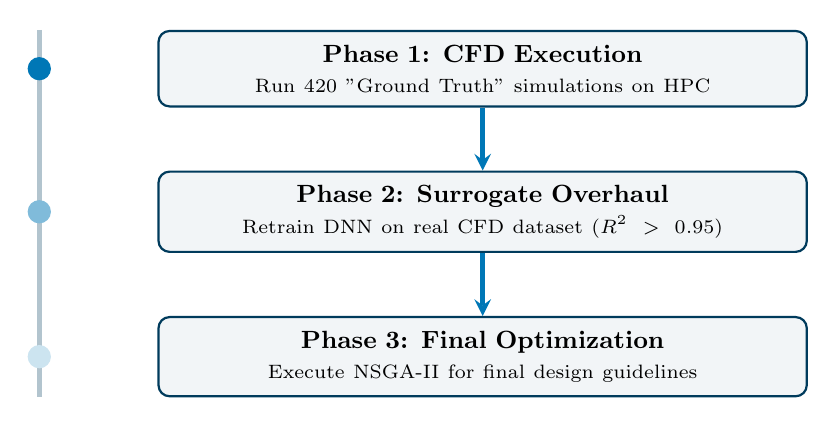
\begin{tikzpicture}[
                node distance=0.8cm,
                phasebox/.style={fill=iitdNavy!5, draw=iitdNavy, thick, rounded corners=4pt,
                                 text width=0.65\linewidth, align=center, font=\small,
                                 inner sep=5pt},
                shadowbox/.style={phasebox, drop shadow={opacity=0.25, shadow xshift=2pt, shadow yshift=-2pt}},
                arrow/.style={->, >=stealth, ultra thick, color=iitdAccent}
            ]
                % Draw shadows manually since drop shadow package might not be loaded
                \node[phasebox] (p1) {\textbf{Phase 1: CFD Execution}\\
                                       \scriptsize Run 420 "Ground Truth" simulations on HPC};
                                       
                \node[phasebox, below=of p1] (p2) {\textbf{Phase 2: Surrogate Overhaul}\\
                                                   \scriptsize Retrain DNN on real CFD dataset ($R^2 > 0.95$)};
                                                   
                \node[phasebox, below=of p2] (p3) {\textbf{Phase 3: Final Optimization}\\
                                                   \scriptsize Execute NSGA-II for final design guidelines};

                \draw[arrow] (p1) -- (p2);
                \draw[arrow] (p2) -- (p3);
                
                % Add a timeline indicator on the left
                \draw[ultra thick, iitdNavy!30] ([xshift=-1.5cm]p1.north west) -- ([xshift=-1.5cm]p3.south west);
                \filldraw[iitdAccent] ([xshift=-1.5cm]p1.west) circle (4pt);
                \filldraw[iitdAccent!50] ([xshift=-1.5cm]p2.west) circle (4pt);
                \filldraw[iitdAccent!20] ([xshift=-1.5cm]p3.west) circle (4pt);
                
            \end{tikzpicture}%
            }
        \end{column}    
    \end{columns}
\end{frame}

% ─── SLIDE 15: REFERENCES ──────────────────────────────────────────────────────
\begin{frame}{Key References}
    \small
    \begin{itemize}
        \item Y.~Tian, T.~Tian, G.~Ren, and J.~Zhang.
        ``Numerical Simulation of Hydrogen Mixing Process in T-Junction Natural Gas Pipeline.''
        \textit{Energies}, vol.~16, no.~1, 2023.

        \vspace{0.8em}
        \item Y.~Su, J.~Li, W.~Guo, Y.~Zhao, et al.
        ``Prediction of Mixing Uniformity of Hydrogen Injection in Natural Gas Pipeline Based on a Deep Learning Model.''
        \textit{Energies}, vol.~15, no.~22, 2022.

        \vspace{0.8em}
        \item A.~K.~Arya, R.~Katiyar, P.~Senthil~Kumar, et al.
        ``A multi-objective model for optimizing hydrogen injected-high pressure natural gas pipeline networks.''
        \textit{Int. Journal of Hydrogen Energy}, vol.~48, 2023.

        \vspace{0.8em}
        \item N.~A.~N.~M.~N.~Azman et al.
        ``Hydrogen-Natural Gas Co-Blending: Performance Analysis with CFD and Static Mixers.''
        \textit{Chemical Engineering Transactions}, vol.~122, 2025.
    \end{itemize}
\end{frame}

% ─── SLIDE 16: THANK YOU ─────────────────────────────────────────────────────
\begin{frame}[plain]
    
\begin{tikzpicture}[remember picture, overlay]
        \fill[left color=iitdDark, right color=iitdAccent!80!iitdNavy]
            (current page.south west) rectangle (current page.north east);
        \fill[white, opacity=0.06]
            ([xshift=-2cm, yshift=-3cm]current page.north east) circle (7cm);
        \fill[white, opacity=0.04]
            ([xshift=3cm, yshift=2cm]current page.south west) circle (5cm);
    \end{tikzpicture}
    \vfill
    \begin{center}
        {\fontsize{28}{34}\selectfont\bfseries\color{white}Thank You}\\[16pt]
        {\Large\color{white}Open for Questions}\\[20pt]
        {\color{white!70}\rule{5cm}{0.5pt}}\\[20pt]
        {\large\color{white}\textbf{Sakhare Yash Balram}}\\[8pt]
        {\normalsize\color{white!90}%
         Department of Chemical Engineering\\
         Indian Institute of Technology Delhi}\\[12pt]
        {\normalsize\color{white!80}%
         \texttt{ch7221496@iitd.ac.in}}
    \end{center}
    \vfill
\end{frame}

\end{document}
